%!TEX root =  main.tex
\section{Experimental evaluation}
\label{sec:experimental-evaluation}

In this section, we present Kernel Paxos and WbCast, the two protocols we compare \libname to (\S\ref{sec:comp}) and
describe the environment where we conducted our experiments (\S\ref{sec:evaluation:setup}).
We conducted three sets of experiments:
in the first set, we seek to understand the effects of message size on \libname (\S\ref{sec:evaluation:micro});
in the second set, we compare Kernel Paxos and WbCast when messages are multicast to a single group (\S\ref{sec:evaluation:broadcast});
finally, we compare the performance of the protocols when messages are multicast to multiple groups (\S\ref{sec:evaluation:multicast}).

\subsection{Competing protocols}
\label{sec:comp}

Kernel Paxos~\cite{esposito2018kernel} is a Multi-Paxos implementation that improves the performance of the original libpaxos library.\footnote{\url{https://bitbucket.org/sciasciad/libpaxos}}
The main idea is to reduce system calls by running Paxos logic directly into the Linux kernel and avoiding the TCP/IP stack. 
We used the original code\footnote{\url{https://github.com/esposem/Kernel_Paxos}} and deployed a single group with three replicas.
We compare \libname to Kernel Paxos because both systems avoid the overhead of the communication stack.
%We have chosen such an implementation because we believe that it has similar features to our library, with optimizations for high throughput and low latency.

White-Box Atomic Multicast~\cite{gotsman2019white}, or WbCast, is a genuine atomic multicast protocol that delivers exceptional performance, thanks to a highly optimized protocol.
%can deliver multi-group messages to the leader of each destination group in three communication steps (four communication steps to the remaining replicas in the destination groups).
 WbCast provides a C-language implementation that uses libevent for communication.\footnote{\url{https://github.com/imdea-software/atomic-multicast}}
 We extended the code to split client and server, and included additional statistics information.


\subsection{Environment setup and configuration parameters}
\label{sec:evaluation:setup}

We conducted all experiments using the CloudLab infrastructure~\cite{DuplyakinATC19cloudlab} with two sets of nodes: 
(a) R320 node for broadcast experiments, equipped with one eight-core Xeon E5-2450 processor running at 2.1GHz, 16 GB of main memory, and a Mellanox FDR CX3 NIC; and (b) XL170 nodes for other experiments, equipped with one ten-core Intel E5-2640v4 processor running at 2.4GHz, 64 GB of main memory, and a Mellanox ConnectX-4 NIC. 
A 10 Gbps network link with around 0.1ms round-trip time connects all nodes running Ubuntu Linux 18.04 with kernel 4.15 an Oracle Java SE Runtime Environment 11. 

In all our experiments, there are client and server processes. 
Clients send requests in a closed-loop, i.e., each client multicasts a message to servers and waits for a response before multicasting the next message. 
In every protocol, each group has 3 processes with in-memory storage.

%We defined three experimental setups:
%in~\S\ref{sec:evaluation:micro} we deployed \libname with a single group and increasing message size;
%\S\ref{sec:evaluation:broadcast} compares \libname with Kernel Paxos and WbCast in a broadcast (single-group) deployment;
%\S\ref{sec:evaluation:multicast} presents a scenario with eight groups contrasting \libname and WbCast with an increasing number of clients and destination groups.

\subsection{The impact of message size}
\label{sec:evaluation:micro}

In this experiment, conducted on XL170 nodes, we measure \libname throughput and latency for different message sizes.
For each message size, from 64 bytes to 64 Kilobytes, we increase the number of clients until the system is saturated, i.e., throughput stops improving while latency raises.
Figure~\ref{fig:1group_message_size} (left) shows that messages up to 4KB long do not impact the overall system throughput, with nearly 250 thousand messages delivered each second. 
As the message size increases, the maximum throughput decreases with 35 thousand messages per second for 64KB messages.
The latency cumulative distribution function (CDF) in Figure~\ref{fig:1group_message_size} (right) exhibits minimum latency variation for messages with up to 2KB, around 8 microseconds at $95^{th}$ percentile. At 4KB messages, the latency slightly go up to around 10 microseconds

\begin{figure*}[htp!]
  \begin{subfigure}{\columnwidth}
    \advance\leftskip+0.08cm
    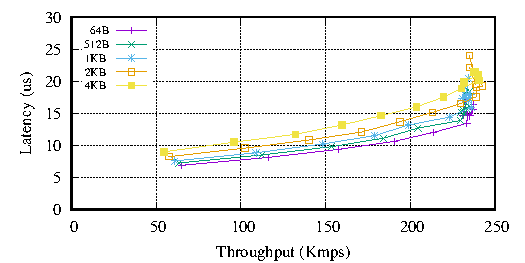
\includegraphics[width=0.97\columnwidth]{figures/benchmark/graphs/figure-performance-vs-size-single-group-up-to-4k}
  \end{subfigure}
  \begin{subfigure}{\columnwidth}
    \advance\leftskip+0.07cm
    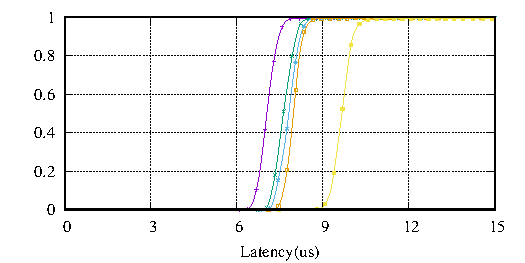
\includegraphics[width=0.96\columnwidth]{figures/benchmark/graphs/figure-performance-vs-size-single-group-cdf-up-to-4k}
  \end{subfigure}
  \begin{subfigure}{\columnwidth}
    \advance\leftskip-0.1cm
    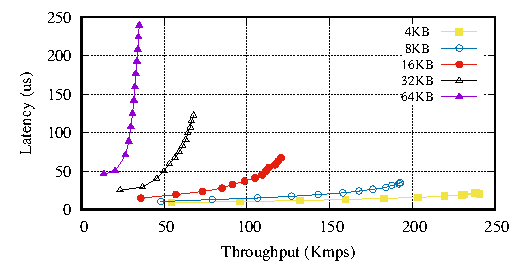
\includegraphics[width=0.99\columnwidth]{figures/benchmark/graphs/figure-performance-vs-size-single-group-from-4k}
  \end{subfigure}
  \begin{subfigure}{\columnwidth}
    \advance\leftskip+0.57cm
    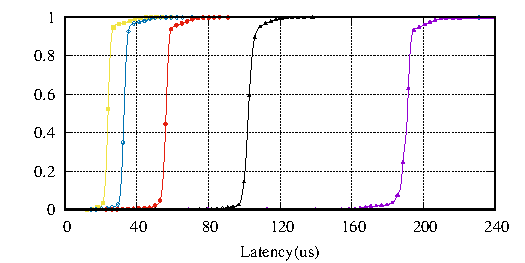
\includegraphics[width=0.96\columnwidth]{figures/benchmark/graphs/figure-performance-vs-size-single-group-cdf-from-4k}
  \end{subfigure}
  \caption{\libname performance with different message sizes: throughput versus latency (left) and latency cumulative distribution function for a single client (right)}
  \label{fig:1group_message_size}
\end{figure*}

\subsection{The performance single-group messages}
\label{sec:evaluation:broadcast}

This experiment assesses how each protocol behaves in a scenario with a single group of three replicas for 64-byte and 1-kilobyte messages.
Figure~\ref{fig:broadcast} (top) shows that, for 64-byte messages, \libname outperforms the competitors with approximately 200 thousand messages per second. 
Kernel Paxos comes close with 170 thousand messages per second, while WbCast saturates sooner, with less than 60 thousand messages per second.
For larger messages, \libname kept the same performance, while the other protocols had the throughput reduced by half.
Figure~\ref{fig:broadcast} (bottom) confirms the superior results for \libname. The median latency for WbCast with small messages and a single client is twenty times greater than the same measurement for our protocol.

\begin{figure}[htp!]
  \begin{subfigure}{\columnwidth}
    \advance\leftskip-0.1cm
    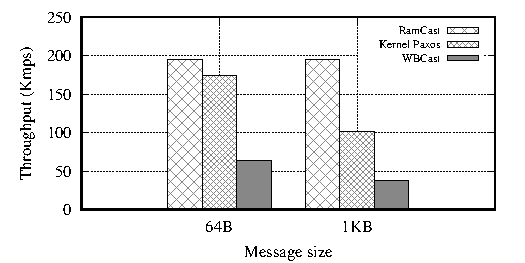
\includegraphics[width=0.99\columnwidth]{figures/benchmark/graphs/figure-compare-single-group-throughput}
  \end{subfigure}
  \begin{subfigure}{\columnwidth}
    \centering
    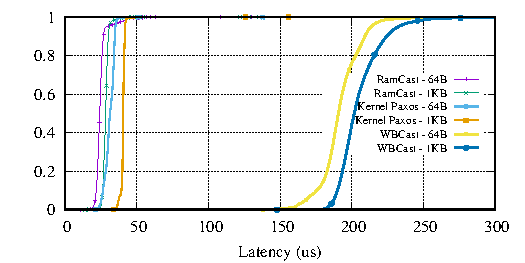
\includegraphics[width=0.95\columnwidth]{figures/benchmark/graphs/figure-compare-single-group-latency-cdf}
  \end{subfigure}
  \caption{Broadcast performance of \libname and competitors: throughput (top) and latency cumulative distribution function for a single client (bottom)}
  \label{fig:broadcast}
\end{figure}


\subsection{The performance multi-group messages}
\label{sec:evaluation:multicast}

The last set of experiments assess \libname behavior in scenarios with up to 8 groups of 3 replicas each, deployed on XL170 machines.
The first experiment comprises executions in which clients send single-group 64-byte messages in setups with 1, 2, 4, and 8 groups.
Figure~\ref{fig:multicast-single-group} (top) shows the aggregated throughput results when the system is saturated. 
\libname outperforms WbCast by a large margin with 227 and 63 thousand messages per second, respectively, for 1 group, and around 1800 and 500 thousand messages per second for 8 groups.
These results also enhance the benefit of genuine atomic multicast algorithms and show that the throughput grows linearly with the number of groups for single-group messages. 
Since groups do not exchange any information when dealing with single-group messages, the latency CDF is the same for a single client, no matter the number of groups in the system, as depicted in Figure~\ref{fig:multicast-single-group} (bottom).

\begin{figure}[htp!]
  \begin{subfigure}{\columnwidth}
    \advance\leftskip-0.25cm
    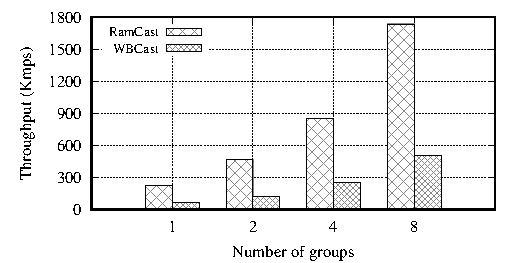
\includegraphics[width=1.01\columnwidth]{figures/benchmark/graphs/figure-genuine-compare-throughput}
  \end{subfigure}
  \begin{subfigure}{\columnwidth}
    \centering
    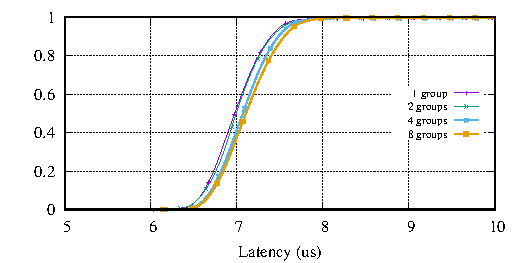
\includegraphics[width=0.95\columnwidth]{figures/benchmark/graphs/figure-genuine-compare-latency-cdf}
  \end{subfigure}
  \caption{Multicast performance of \libname and WbCast for single group messages: throughput (top) and latency cumulative distribution function of a \libname's single client (bottom)}
  \label{fig:multicast-single-group}
\end{figure}

The next experiment evaluates how the protocols behave regarding multi-group messages. 
In setups with 1, 2, 4, and 8 groups, clients send 64-byte messages addressed to all the groups.
\libname's maximum throughput is greater than WbCast's in every configuration with 233, 145, 80, and 40 thousand messages per second for 1, 2, 4, and 8 destination groups against 63, 50, 35, and 27 thousand for WbCast, as shown in Figure~\ref{fig:multicast-multi-group} (top).
The difference is even more expressive if we consider the latency for a single client, i.e., when both protocols are contention-free. Figure~\ref{fig:multicast-multi-group} (middle) shows that the latency CDF for \libname with values of 8, 46, 78 and 150~microseconds for 1, 2, 4, and 8 destination groups if we consider the $95^{th}$ percentile. 
The equivalent values for WbCast are 214, 445, 673, and 1055~microseconds, representing 20 to 7 times slower delivery times when compared to \libname's.

\begin{figure}[htp!]
  \begin{subfigure}{\columnwidth}
    \advance\leftskip-0.1cm
    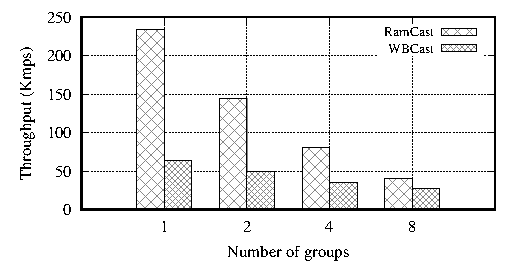
\includegraphics[width=0.99\columnwidth]{figures/benchmark/graphs/figure-multi-dest-compare-throughput}
  \end{subfigure}
  \begin{subfigure}{\columnwidth}
    \centering
    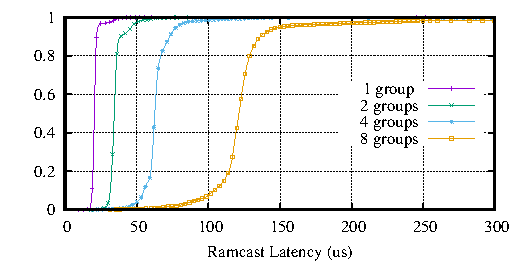
\includegraphics[width=0.95\columnwidth]{figures/benchmark/graphs/figure-multi-dest-compare-latency-cdf-ramcast}
  \end{subfigure}
  \begin{subfigure}{\columnwidth}
    \centering
    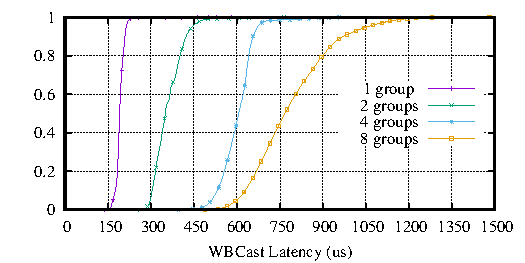
\includegraphics[width=0.95\columnwidth]{figures/benchmark/graphs/figure-multi-dest-compare-latency-cdf-wbcast}
  \end{subfigure}
  \caption{Performance comparison of \libname and WbCast for multi-groups message: throughput (top) and latency cumulative distribution function of \libname's (middle) and WbCast's single client (bottom)}
  \label{fig:multicast-multi-group}
\end{figure}
